\documentclass[11pt]{amsart}
\usepackage[T1]{fontenc}
\usepackage{lmodern}
\usepackage[margin=1.1in]{geometry}
\usepackage[numbers,sort&compress]{natbib}
\usepackage{amssymb,amsmath,mathtools}
\usepackage{graphicx}
\usepackage{booktabs}
\usepackage{array}
\usepackage[hidelinks]{hyperref}
\usepackage{xcolor}
\usepackage{tikz}
\usetikzlibrary{positioning}
\setlength{\emergencystretch}{1.5em}
\renewcommand{\topfraction}{0.9}
\renewcommand{\textfraction}{0.1}
\renewcommand{\floatpagefraction}{0.8}

\newtheorem{theorem}{Theorem}[section]
\newtheorem{lemma}[theorem]{Lemma}
\newtheorem{proposition}[theorem]{Proposition}
\theoremstyle{definition}
\newtheorem{construction}[theorem]{Construction}
\newtheorem{remark}[theorem]{Remark}

\newcommand{\F}{\mathbb{F}}
\newcommand{\Z}{\mathbb{Z}}
\newcommand{\srg}{\mathrm{srg}}
\newcommand{\Cay}{\mathrm{Cay}}
\newcommand{\Aut}{\mathrm{Aut}}
\newcommand{\LS}{\mathrm{LS}}
\newcommand{\NL}{\mathrm{NL}}
\newcommand{\todo}[1]{\textcolor{red}{[TODO: #1]}}

\title[Strongly regular graphs on 1296 vertices]{New strongly regular graphs on 1296 vertices\\ from partial difference sets in $\F_{16}\times\F_{81}$}
\author{Dylan Plummer}
\address{Case Western Reserve University}
\email{dylan.plummer@case.edu}
\date{\today}

\begin{document}

\begin{abstract}
We construct strongly regular graphs with parameters $(1296,560,244,240)$ and $(1296,592,268,272)$, for which no construction was previously known. We also construct the first vertex-transitive graphs with parameters $(1296,595,274,272)$, a parameter set realised independently by Kova\v{l}. All are Cayley graphs of $\Z_2^4\times\Z_3^4$, realised as the additive group of $\F_{16}\times\F_{81}$, whose connection sets are unions of orbits of a small group of field multiplications and a Galois map. We find $10$, $4$ and $4$ pairwise non-isomorphic graphs with the three parameter sets. The connection sets were found by an exact constraint-programming search for partial difference sets in products of finite fields, which generalises Kova\v{l}'s search in $\F_4\times\F_{81}$ for $\srg(324,136,58,56)$. The three families are linked by spreads of Delsarte cliques. Some of the graphs with the first parameter set arise from an $\srg(1296,665,340,342)$ by deleting three pairwise orthogonal spreads, a configuration that Kova\v{l} looked for in graphs from Bush-type Hadamard matrices, and the graphs with the third parameter set arise by deleting two. None of the graphs with Latin square parameters is the graph of an orthogonal array. In the first graph every coset of $\F_{81}$ induces the Brouwer--Haemers graph $\srg(81,20,1,6)$.
\end{abstract}

\maketitle

%=====================================================================
\section{Introduction}

A strongly regular graph $\srg(v,k,\lambda,\mu)$ is a $k$-regular graph on $v$ vertices, neither complete nor edgeless, in which any two adjacent vertices have exactly $\lambda$ common neighbours and any two distinct non-adjacent vertices exactly $\mu$. Brouwer maintains an online table of feasible parameter sets~\cite{BrouwerTable}; see also the monograph of Brouwer and Van Maldeghem~\cite{BvM2022}. All three parameter sets of Theorems~\ref{thm:main} and~\ref{thm:595} were marked there as open when this work began.

A standard route to strongly regular graphs is through partial difference sets (PDS). If $D$ is a $(v,k,\lambda,\mu)$-PDS in a group $G$ with $D=D^{(-1)}$ and $1\notin D$, then the Cayley graph $\Cay(G,D)$ is an $\srg(v,k,\lambda,\mu)$~\cite{Ma1994}. Brady~\cite{Brady2025} turned this into a systematic computational programme aimed at \emph{new} strongly regular graphs. A local search over all groups of order at most $147$ found PDSs with 62 parameter sets in 1254 groups, including the first constructions of $\srg(144,52,16,20)$ and $\srg(147,66,25,33)$.

Recently Kova\v{l}~\cite[Section~5]{KovalNew} realised the Latin square parameters $\LS_8(18)=(324,136,58,56)$ and the negative Latin square parameters $\NL_6(18)$ and $\NL_7(18)$ by PDSs in $\Z_2^2\times\Z_3^4$. One of these is a cyclotomic construction in the additive group of $\F_4\times\F_{81}$: the connection set is invariant under multiplication by the fourth roots of unity $\mu_4\le\F_{81}^*$, and each of its four slices $D_a$, $a\in\F_4$, is a union of cyclotomic classes of index~$20$ in~$\F_{81}$~\cite[Construction~5.4]{KovalNew}.

This paper replaces $\F_4$ by $\F_{16}$ and searches systematically over the symmetry groups that the product structure provides (Section~\ref{sec:search}). On $1296=36^2$ vertices this produces the following.

\begin{theorem}\label{thm:main}
There exist strongly regular graphs with parameters
\[
 (1296,560,244,240)\ \ (\LS_{16}(36)) \qquad\text{and}\qquad (1296,592,268,272)\ \ (\NL_{16}(36)).
\]
There are at least $10$ pairwise non-isomorphic graphs with the first parameter set and at least $4$ with the second. All of them are vertex-transitive Cayley graphs of $\Z_2^4\times\Z_3^4$.
\end{theorem}

The parameters $(1296,595,274,272)=\LS_{17}(36)$ were realised independently by Kova\v{l}~\cite{KovalMultiOrbit}, with six graphs, none of them vertex-transitive. Our search gives the first vertex-transitive examples.

\begin{theorem}\label{thm:595}
There are at least $4$ pairwise non-isomorphic vertex-transitive strongly regular graphs with parameters $(1296,595,274,272)$. They are Cayley graphs of $\Z_2^4\times\Z_3^4$, so their connection sets are abelian partial difference sets with these parameters, and none of them is isomorphic to a graph of~\cite{KovalMultiOrbit}.
\end{theorem}

The three families are related by deleting spreads of Delsarte cliques (Section~\ref{sec:spreads}). Two of the graphs with parameters $\LS_{16}(36)$ arise from a Cayley graph with parameters $\LS_{19}(36)$ by deleting three pairwise orthogonal spreads. Kova\v{l} looked for this configuration in graphs from Bush-type Hadamard matrices~\cite[Section~4.10]{KovalMultiOrbit}. The graphs of Theorem~\ref{thm:595} arise in the same way by deleting two.

%=====================================================================
\section{Preliminaries}

\subsection{Latin square type parameters}
For $n\ge2$ and $1\le m\le n+1$ the \emph{Latin square} and \emph{negative Latin square} parameters are
\begin{align*}
\LS_m(n)&=\bigl(n^2,\,m(n-1),\,n-2+(m-1)(m-2),\,m(m-1)\bigr),\\
\NL_m(n)&=\bigl(n^2,\,m(n+1),\,-n+m^2+3m,\,m(m+1)\bigr).
\end{align*}
An $\LS_m(n)$ graph has eigenvalues $n-m$ and $-m$; an $\NL_m(n)$ graph has eigenvalues $m$ and $m-n$. The graph of an orthogonal array $\mathrm{OA}(n,m)$ (equivalently, of $m-2$ mutually orthogonal Latin squares of order $n$) is an $\LS_m(n)$ graph, and every edge of it lies in a clique of size $n$. For $n=36$ only eight MOLS are known, so orthogonal arrays give $\LS_m(36)$ graphs only for $m\le10$ (and their complements).

\subsection{Partial difference sets and characters}
Let $G$ be a finite abelian group, written additively, and let $D\subseteq G\setminus\{0\}$ with $D=-D$ and $|D|=k$. Let $(v,k,\lambda,\mu)$ be feasible with integral eigenvalues $r>s$, the roots of $x^2-(\lambda-\mu)x-(k-\mu)$.

\begin{lemma}[{see \cite{Ma1994}}]\label{lem:char}
$D$ is a $(v,k,\lambda,\mu)$-PDS if and only if $\chi(D)=\sum_{d\in D}\chi(d)\in\{r,s\}$ for every non-principal character $\chi$ of $G$.
\end{lemma}

\begin{lemma}[{\cite[Theorem~4.1]{Ma1994}}]\label{lem:mult}
Let $D$ be a regular PDS in an abelian group $G$ (that is, $0\notin D=-D$). If $(\lambda-\mu)^2+4(k-\mu)$ is a perfect square, then $tD=D$ for every integer $t$ coprime to $|G|$.
\end{lemma}
In particular, a PDS with integral eigenvalues is a union of orbits of the multiplier group $\{x\mapsto tx:\gcd(t,|G|)=1\}$. Any additional group of automorphisms that we impose on $D$ can therefore be taken to contain the multipliers, with no loss of generality.

%=====================================================================
\section{The search}\label{sec:search}

\subsection{Products of finite fields}
Let $G=\F_{q_1}\times\cdots\times\F_{q_t}$ (additive group) with $q_i=p_i^{e_i}$ and $v=\prod q_i$. Every $\boldsymbol\gamma=(\gamma_1,\dots,\gamma_t)\in\prod\F_{q_i}^*$ acts on $G$ by $(a_i)\mapsto(\gamma_ia_i)$, and every $\boldsymbol\sigma=(\sigma_1,\dots,\sigma_t)$ with $\sigma_i\in\mathrm{Gal}(\F_{q_i}/\F_{p_i})$ acts by $(a_i)\mapsto(\sigma_i(a_i))$. Both are group automorphisms. For a subgroup $S\le\prod\F_{q_i}^*$ and an optional Galois element $\boldsymbol\sigma$ we let
\[
K(S,\boldsymbol\sigma)=\bigl\langle\, S,\ \boldsymbol\sigma,\ \{x\mapsto tx:\gcd(t,v)=1\}\,\bigr\rangle\le\Aut(G).
\]
A \emph{model} is a pair $(S,\boldsymbol\sigma)$. Its solutions are the $K(S,\boldsymbol\sigma)$-invariant PDSs in $G$ with prescribed parameters.

\subsection{An exact formulation}
Let $O_1,\dots,O_n$ be the orbits of $K=K(S,\boldsymbol\sigma)$ on $G$, and let $\Omega_1,\dots,\Omega_m$ be the orbits of the dual action of $K$ on the character group $\widehat G$. The value $\chi(O_i)$ depends only on the dual orbit of $\chi$. Because $K$ contains all multipliers, $\chi(O_i)$ is fixed by $\mathrm{Gal}(\mathbb{Q}(\zeta_{\exp G})/\mathbb{Q})$, so $c_{ji}=\chi_j(O_i)\in\Z$ for a representative $\chi_j\in\Omega_j$. By Lemma~\ref{lem:char}, $K$-invariant $(v,k,\lambda,\mu)$-PDSs correspond exactly to the $0/1$ solutions $(x,b)$ of
\[
\sum_i |O_i|\,x_i=k,\qquad x_{\{0\}}=0,\qquad \sum_i c_{ji}\,x_i=s+(r-s)\,b_j\quad(\Omega_j\ne\{1\}),\qquad \sum_j|\Omega_j|\,b_j=f,
\]
where $f$ is the multiplicity of the eigenvalue $r$; the last equation is implied by the others but helps the solver. We solve this integer program with the CP-SAT solver of OR-Tools~\cite{CPSAT}. Every solution is checked independently by the full identity $A^2=kI+\lambda A+\mu(J-I-A)$ for $A$ the adjacency matrix of $\Cay(G,D)$.

\subsection{Relation to Kova\v{l}'s search}
Kova\v{l}'s cyclotomic search on $\F_4\times\F_{81}$~\cite[Section~5.4]{KovalNew} is the case $(q_1,q_2)=(4,81)$ of this scheme. There $S$ runs over the $16$ subgroups of even order of the cyclic group $\F_4^*\times\F_{81}^*\cong C_{240}$, and the Galois part over the $8$ subgroups of $\mathrm{Gal}(\F_4/\F_2)\times\mathrm{Gal}(\F_{81}/\F_3)$. For $(q_1,q_2)=(16,81)$ the group $\F_{16}^*\times\F_{81}^*\cong C_{15}\times C_{80}$ is not cyclic, and we let $S$ run over all of its $80$ subgroups. Here $S$ need not have even order, because $-1$ is among the multipliers. $\boldsymbol\sigma$ runs over the trivial map and the $15$ maps $(a,b)\mapsto(a^{2^u},b^{3^w})$ with $(u,w)\ne(0,0)$. This gives $1280$ models. The $1251$ models with at most $200$ orbits were each tested against every parameter set $(1296,k,\lambda,\mu)$ with $k\le 648$ and integral eigenvalues that was open in Brouwer's table; complements cover the rest. Section~\ref{sec:graphs} presents the solutions, which have the three parameter sets of Theorems~\ref{thm:main} and~\ref{thm:595}. The same scheme was also run on other products of finite fields; the solver settings and the coverage of the search, which is still running, are recorded in the data repository.

%=====================================================================
\section{The graphs}\label{sec:graphs}

Throughout, $\F_{16}=\F_2[x]/(x^4+x^3+1)$ and $\F_{81}=\F_3[y]/(y^4+y^3+2)$, with primitive elements $\alpha=x$ and $\beta=y$. Vertices are pairs $(a,b)\in\F_{16}\times\F_{81}$, and $(a,b)\sim(a',b')$ if and only if $(a-a',b-b')\in D$.

\begin{construction}[Graph I]\label{con:I}
Let
\[
\begin{aligned}
S_I=\{&(0,0),(0,2),(0,6),(0,11),(0,13),(0,14),(0,17),(0,18),(0,19),\\
&(1,3),(1,6),(1,7),(1,8),(1,10),(1,11),(1,13),(1,15),(1,19),\\
&(2,1),(2,2),(2,5),(2,9),(2,10),(2,11),(2,13),(2,16),(2,17)\}\subseteq\Z_3\times\Z_{20},
\end{aligned}
\]
and
\begin{multline*}
D_I=\{(0,\beta^{j}):j\equiv0\pmod 4\}\\
\cup\ \bigl\{(\alpha^i,\beta^j):0\le i<15,\ 0\le j<80,\ \bigl(i\bmod 3,\ (j-4\lfloor i/3\rfloor)\bmod 20\bigr)\in S_I\bigr\}.
\end{multline*}
Then $|D_I|=20+27\cdot20=560$. $D_I$ is invariant under $(a,b)\mapsto(\alpha^3a,\beta^4b)$, which has order $20$ and whose tenth power is $-1$, and under $(a,b)\mapsto(a^2,b^{27})$.
\end{construction}

\begin{construction}[Graph II]\label{con:II}
Let $J_a\subseteq\Z_{20}$ for $a\in\F_{16}$ be given by Table~\ref{tab:J}, and
\[
D_{II}=\{(a,\beta^j):a\in\F_{16},\ 0\le j<80,\ j\bmod 20\in J_a\}.
\]
Then $|D_{II}|=4\,(13+15\cdot9)=592$. $D_{II}$ is invariant under multiplication by $\mu_4=\langle\beta^{20}\rangle$ on the second coordinate and under $(a,b)\mapsto(a^2,b^3)$. Each slice $D_a=\{b:(a,b)\in D_{II}\}$ is a union of the cyclotomic classes $C_j=\beta^j\mu_4$ of index $20$. This is the shape of Kova\v{l}'s Construction~5.4 in~\cite{KovalNew}, with $\F_4$ replaced by $\F_{16}$.
\end{construction}

\begin{construction}[Graph III]\label{con:III}
Let $J'_a\subseteq\Z_{20}$ for $a\in\F_{16}$ be given by Table~\ref{tab:J}, and
\[
D_{III}=\{(a,\beta^j):a\in\F_{16},\ 0\le j<80,\ j\bmod 20\in J'_a\}\ \cup\ \bigl(\F_4^*\times\{0\}\bigr),
\]
where $\F_4^*=\{1,\alpha^5,\alpha^{10}\}$. Then $|D_{III}|=4\,(7+3\cdot11+12\cdot9)+3=595$. $D_{III}$ is invariant under multiplication by $\mu_4$ on the second coordinate and under $(a,b)\mapsto(a^2,b^3)$. The three slices with $|J'_a|=11$ are those with $a\in\F_4^*$.
\end{construction}

\begin{table}[ht]
\centering\small
\caption{The sets $J_a$ of Construction~\ref{con:II} and $J'_a$ of Construction~\ref{con:III}.}\label{tab:J}
\begin{tabular}{>{$}l<{$}>{$}l<{$}>{$}l<{$}}
\toprule
a & J_a\ (\Gamma_{II}) & J'_a\ (\Gamma_{III})\\
\midrule
0 & \{0,1,3,4,7,8,9,11,12,13,16,17,19\} & \{0,4,5,8,12,15,16\}\\
\alpha^0 & \{0,2,6,11,13,14,17,18,19\} & \{0,2,5,6,11,13,14,15,17,18,19\}\\
\alpha^1 & \{4,6,7,10,11,12,13,15,19\} & \{5,9,10,12,13,14,16,18,19\}\\
\alpha^2 & \{1,5,10,12,13,16,17,18,19\} & \{2,7,8,10,14,15,16,17,19\}\\
\alpha^3 & \{1,2,7,9,10,14,15,18,19\} & \{3,4,5,6,10,12,13,14,19\}\\
\alpha^4 & \{3,8,10,11,14,15,16,17,19\} & \{1,2,4,5,6,8,10,11,17\}\\
\alpha^5 & \{0,1,5,6,9,13,14,15,17\} & \{0,2,3,4,6,7,11,14,16,18,19\}\\
\alpha^6 & \{1,2,3,5,6,7,10,14,17\} & \{2,9,10,12,15,16,17,18,19\}\\
\alpha^7 & \{0,1,5,6,7,8,10,13,14\} & \{0,2,4,5,9,10,11,16,17\}\\
\alpha^8 & \{2,4,5,8,9,10,11,13,17\} & \{3,4,6,10,11,12,13,15,18\}\\
\alpha^9 & \{3,5,6,7,9,10,13,14,18\} & \{1,2,4,8,10,11,13,15,18\}\\
\alpha^{10} & \{0,2,3,5,7,11,15,18,19\} & \{0,1,2,6,8,9,12,13,14,17,18\}\\
\alpha^{11} & \{0,2,7,9,10,11,15,16,18\} & \{0,3,8,10,12,14,15,17,19\}\\
\alpha^{12} & \{1,2,3,6,9,10,11,15,18\} & \{5,6,7,8,10,11,14,16,17\}\\
\alpha^{13} & \{0,3,5,6,9,10,12,14,17\} & \{0,1,4,5,10,13,16,18,19\}\\
\alpha^{14} & \{0,1,2,3,4,10,15,18,19\} & \{0,6,7,8,10,11,12,13,15\}\\
\bottomrule
\end{tabular}
\end{table}

\begin{theorem}\label{thm:graphs}
$D_I$, $D_{II}$ and $D_{III}$ are partial difference sets in $(\F_{16}\times\F_{81},+)\cong\Z_2^4\times\Z_3^4$ with parameters $(1296,560,244,240)$, $(1296,592,268,272)$ and $(1296,595,274,272)$. Consequently the Cayley graphs $\Gamma_I$, $\Gamma_{II}$, $\Gamma_{III}$ of $\F_{16}\times\F_{81}$ with these connection sets are strongly regular, with spectra $560^1\,20^{560}\,(-16)^{735}$, $592^1\,16^{703}\,(-20)^{592}$ and $595^1\,19^{595}\,(-17)^{700}$.
\end{theorem}

\begin{proof}
All three sets satisfy $D=-D$ and $0\notin D$. The identity $A^2=kI+\lambda A+\mu(J-I-A)$ was verified exhaustively, by counting the common neighbours of all $\binom{1296}{2}$ vertex pairs of $\Cay(G,D)$ (Section~\ref{sec:verification}). As a consistency check, all $1295$ non-principal character values were computed numerically. They take exactly the two values $r,s$ allowed by Lemma~\ref{lem:char}, with the multiplicities of the stated spectrum.
\end{proof}

\begin{remark}
Like Kova\v{l}'s Construction~5.4, these proofs are computational. A hand proof via Gauss periods, in the style of~\cite[Section~5.3]{KovalNew}, should be possible, since the character values are sums of Gauss periods of $\F_{16}$ and $\F_{81}$. % \todo{attempt a hand proof for Construction~\ref{con:II}.}

\end{remark}

\subsection{Further graphs}
Table~\ref{tab:classes} lists all isomorphism classes found. Graphs I.7--I.10, II.1--II.4 and III.1--III.4 come from the same four models $(S,\boldsymbol\sigma)$, with $S=\langle(1,\beta^{20})\rangle\cong\mu_4$ and one of four Galois maps. Each of these four models has solutions for all three parameter sets. Kova\v{l}'s six graphs with parameters $(1296,595,274,272)$~\cite{KovalMultiOrbit} have automorphism groups of orders $2903040$, $3456$, $31104$, $19584$, $1$ and $1$, and none is vertex-transitive. Comparing nauty canonical forms~\cite{McKayPiperno2014} shows that none of them is isomorphic to III.1--III.4, which proves the last claim of Theorem~\ref{thm:595}. The connection sets of all eighteen graphs are in the data repository (see Data availability).

\begin{table}[ht]
\centering\small
\caption{Non-isomorphic graphs found, with $|\Aut\Gamma|$ computed by nauty, the order of the multiplicative stabiliser $\mathrm{Stab}(D)=\{\gamma\in\F_{16}^*\times\F_{81}^*:\gamma D=D\}$ of the connection set, the clique number $\omega$, and the model in which each graph was first found. A multiplicative generator $(\alpha^x,\beta^y)$ acts by $(a,b)\mapsto(\alpha^xa,\beta^yb)$, and a Galois map is written by its action on $(a,b)$.}\label{tab:classes}
\begin{tabular}{llrrrl}
\toprule
graph & parameters & $|\Aut\Gamma|$ & $|\mathrm{Stab}(D)|$ & $\omega$ & model $(S,\boldsymbol\sigma)$\\
\midrule
I.1 & $(1296,560,244,240)$ & 103680 & 20 & 12 & $\langle(\alpha^3,\beta^4)\rangle$, $(a^2,b^{27})$ \\
I.2 & & 51840 & 20 & 12 & $\langle(\alpha^3,\beta^{12})\rangle$, $(a^4,b^{9})$ \\
I.3 & & 51840 & 10 & 12 & $\langle(\alpha^3,\beta^{16})\rangle$, $(a^2,b^{27})$ \\
I.4 & & 51840 & 20 & 12 & $\langle(\alpha^3,\beta^{12})\rangle$, none \\
I.5 & & 25920 & 20 & 12 & $\langle(\alpha^3,\beta^{36})\rangle$, none \\
I.6 & & 25920 & 20 & 12 & $\langle(\alpha^3,\beta^{4})\rangle$, none \\
I.7 & & 20736 & 4 & 12 & $\langle(1,\beta^{20})\rangle$, $(a^2,b^{3})$ \\
I.8 & & 20736 & 4 & 15 & $\langle(1,\beta^{20})\rangle$, $(a^2,b^{27})$ \\
I.9 & & 20736 & 4 & 12 & $\langle(1,\beta^{20})\rangle$, $(a^8,b^{3})$ \\
I.10 & & 20736 & 4 & 14 & $\langle(1,\beta^{20})\rangle$, $(a^8,b^{27})$ \\
\midrule
II.1 & $(1296,592,268,272)$ & 20736 & 4 & 13 & $\langle(1,\beta^{20})\rangle$, $(a^2,b^{3})$ \\
II.2 & & 20736 & 4 & 12 & $\langle(1,\beta^{20})\rangle$, $(a^2,b^{27})$ \\
II.3 & & 20736 & 4 & 12 & $\langle(1,\beta^{20})\rangle$, $(a^8,b^{3})$ \\
II.4 & & 20736 & 4 & 12 & $\langle(1,\beta^{20})\rangle$, $(a^8,b^{27})$ \\
\midrule
III.1 & $(1296,595,274,272)$ & 20736 & 4 & 24 & $\langle(1,\beta^{20})\rangle$, $(a^2,b^{3})$ \\
III.2 & & 20736 & 4 & 24 & $\langle(1,\beta^{20})\rangle$, $(a^2,b^{27})$ \\
III.3 & & 20736 & 4 & 24 & $\langle(1,\beta^{20})\rangle$, $(a^8,b^{3})$ \\
III.4 & & 20736 & 4 & 24 & $\langle(1,\beta^{20})\rangle$, $(a^8,b^{27})$ \\
\bottomrule
\end{tabular}
\end{table}

Graphs I.1, II.1 and III.1 are $\Gamma_I$, $\Gamma_{II}$ and $\Gamma_{III}$ of Constructions~\ref{con:I}--\ref{con:III}. All eighteen graphs are vertex-transitive, being Cayley graphs. The counts are lower bounds, since the search is not exhaustive.

%=====================================================================
\section{Properties}\label{sec:properties}

\subsection{Clique numbers}
In the graph of an $\mathrm{OA}(36,m)$ every edge lies in a $36$-clique, which attains the Delsarte bound $1-k/s=36$. We computed the clique numbers $\omega$ of all eighteen graphs exactly (Table~\ref{tab:classes}). Since $\Gamma$ is vertex-transitive, a maximum clique may be taken to contain $(0,0)$ and an edge $\{(0,0),x\}$, so $\omega(\Gamma)=2+\max_x\omega(\Gamma(0,0)\cap\Gamma(x))$. Here $x$ runs over representatives of the orbits of the known automorphisms fixing $(0,0)$ on its neighbours. Each common neighbourhood has $\lambda$ vertices, and its clique number was computed exactly with Cliquer (through igraph). A clique of size $\omega$ was exhibited in each case, and the values for I.1 and I.8 were confirmed with a second exact solver (networkx). The clique numbers are $12$, $14$ or $15$ for the graphs I, $12$ or $13$ for the graphs II and $24$ for the graphs III. They are far below the Delsarte bounds, which are $36$ for I and III and $30$ for II. In particular none of the graphs I and III is the graph of an orthogonal array, and they say nothing about the existence of $14$ or $15$ MOLS of order $36$.

\subsection{Ring structure}
Let $R_a=\{a\}\times\F_{81}$ for $a\in\F_{16}$; we call these sets \emph{rings}. Since they are the cosets of a subgroup, $\{R_a\}$ is an equitable partition of every Cayley graph of $G$.

\begin{proposition}\label{prop:rings}
In $\Gamma_I$ each ring induces the Brouwer--Haemers graph $\srg(81,20,1,6)$~\cite{BrouwerHaemers1992}, namely the cyclotomic graph $\Cay(\F_{81},\langle\beta^4\rangle)$, and every vertex has exactly $36$ neighbours in each of the other $15$ rings. In $\Gamma_{II}$ each ring induces a $52$-regular graph that is not strongly regular, and every vertex has exactly $36$ neighbours in each other ring. In $\Gamma_{III}$ each ring induces a $28$-regular graph that is not strongly regular. A vertex of $R_a$ has $45$ neighbours in each of the three rings $R_{a+c}$, $c\in\F_4^*$, and $36$ in each of the other twelve rings.
\end{proposition}

\begin{proof}
The subgraph induced on $R_a$ is $\Cay(\F_{81},D\cap(\{0\}\times\F_{81}))$, and $D_I\cap(\{0\}\times\F_{81})=\{0\}\times\langle\beta^4\rangle$. The cyclotomic graph of index $4$ on $\F_{81}$ is the Brouwer--Haemers graph. The remaining counts are $|D\cap(\{a\}\times\F_{81})|$ for $a\neq0$, read off from the constructions. For $\Gamma_{II}$, adjacent pairs in a ring have $31$ or $37$ common neighbours inside the ring, and for $\Gamma_{III}$ they have $1$, $7$ or $13$.
\end{proof}

The quotient matrix of the partition $\{R_a\}$ is $cI+36(J-I)$ with $c=20$ for $\Gamma_I$ and $c=52$ for $\Gamma_{II}$. Its eigenvalues are $c+15\cdot36=k$ and $c-36$, which equals $-16$ for $\Gamma_I$ and $16$ for $\Gamma_{II}$, as they must be. For $\Gamma_{III}$ the quotient matrix is not of this form, because the subfield $\F_4$ singles out three rings, and it has eigenvalues $595$, $19$ and $-17$. Figure~\ref{fig:rings} illustrates the ring structure, and its right-hand panels zoom into a single ring. An interactive visualisation of all eighteen graphs, including their adjacency matrices, is in the data repository. The ring graphs of $\Gamma_{II}$ show that strong regularity of $\Gamma$ does not require strongly regular rings. For two vertices of the same ring of $\Gamma_{II}$, the number of common neighbours inside the ring varies ($31$ or $37$ for adjacent pairs, $26$, $32$ or $38$ for non-adjacent ones), and the other $15$ rings contribute exactly the complementary amount.

\begin{figure}[p]
\centering
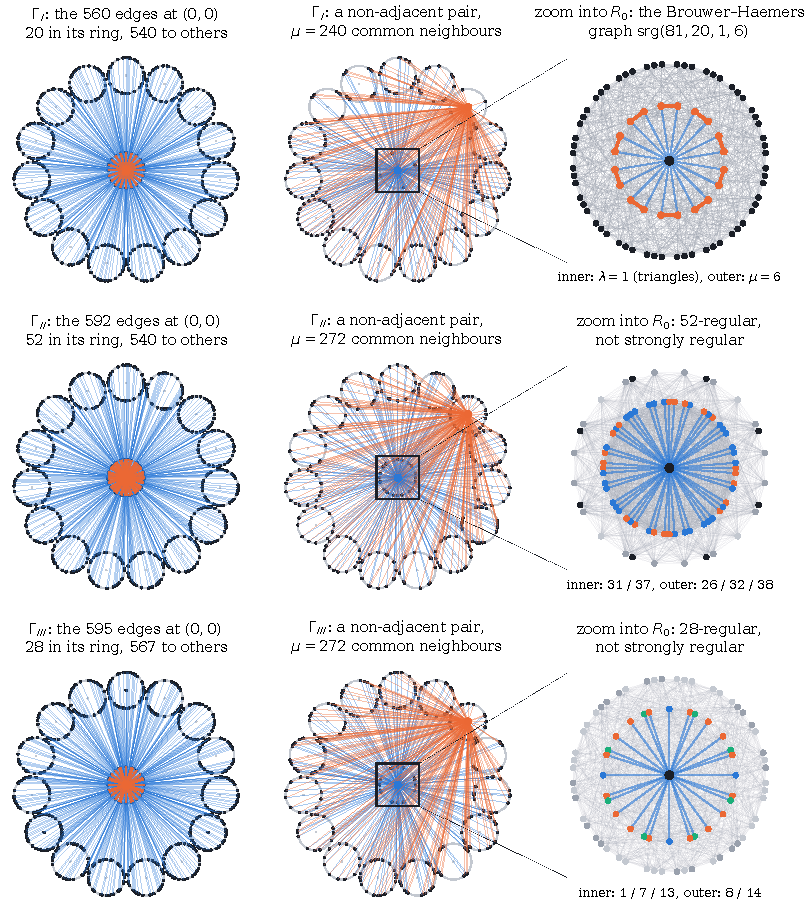
\includegraphics[height=0.69\textheight,width=\textwidth,keepaspectratio]{figures/rings.pdf}
\caption{Rows: $\Gamma_I$, $\Gamma_{II}$, $\Gamma_{III}$. Left and middle: all $1296$ vertices in the ring layout. Ring $R_{\alpha^i}$ is centred at angle $2\pi i/15$ and $R_0$ is in the middle; within a ring, $(a,\beta^j)$ sits at angle $2\pi j/80$ with $(a,0)$ at its centre. Left: the edges at $(0,0)$, orange inside its ring and blue to other rings. Middle: a non-adjacent pair, $(0,0)$ (blue) and a vertex of $R_{\alpha^{13}}$ (orange), with the edges from both to their $\mu$ common neighbours (black dots). Right: the subgraph induced on the framed ring $R_0$. Here $(0,0)$ is in the centre, its neighbours in the ring on the inner circle and its non-neighbours in the ring on the outer circle. Each vertex is coloured by its number of common neighbours with $(0,0)$ inside the ring. In $\Gamma_I$ these numbers are constant, $\lambda=1$ and $\mu=6$: the ring is the Brouwer--Haemers graph $\srg(81,20,1,6)$, and the $20$ neighbours of $(0,0)$ form ten triangles with it. In $\Gamma_{II}$ and $\Gamma_{III}$ the ring graphs are $52$- and $28$-regular but not strongly regular. The inner numbers are $31$ or $37$ (blue, orange) for $\Gamma_{II}$ and $1$, $7$ or $13$ (blue, orange, green) for $\Gamma_{III}$. The outer numbers are $26$, $32$ or $38$ and $8$ or $14$ (light to dark).}\label{fig:rings}
\end{figure}

\subsection{Spread structure}\label{sec:spreads}
Following Haemers and Tonchev~\cite{HaemersTonchev1996}, a \emph{spread} of a strongly regular graph is a partition of its vertex set into Delsarte cliques, that is, cliques of size $1-k/s$. Two spreads are \emph{orthogonal} if every clique of one meets every clique of the other in exactly one vertex. Kova\v{l}~\cite[Lemma~4.1]{KovalMultiOrbit}, building on~\cite[Proposition~4.1]{HaemersTonchev1996}, showed the following: if $\mathcal S_1,\dots,\mathcal S_j$ are pairwise orthogonal spreads of a primitive strongly regular graph with the parameters of $\LS_t(n)$, $j<t$, then deleting the edges inside all their cliques leaves a strongly regular graph with the parameters of $\LS_{t-j}(n)$. Kova\v{l} constructed $\LS_{n/2-1}(n)$ graphs this way, by deleting two orthogonal spreads from $\LS_{n/2+1}(n)$ graphs coming from Bush-type Hadamard matrices, and asked whether a third orthogonal spread can be deleted, which for $n=36$ would give the parameters $\LS_{16}(36)=(1296,560,244,240)$ of $\Gamma_I$~\cite[Section~4.10]{KovalMultiOrbit}.

In a Cayley graph $\Cay(G,E)$, a subgroup $U$ of order $36$ with $U\setminus\{0\}\subseteq E$ makes the cosets of $U$ cliques of size $36$. For an $\LS_{19}(36)$ graph these are Delsarte cliques, since $1-k/s=1+665/19=36$. So the cosets of $U$ form a spread, and the spreads of two such subgroups $U,V$ are orthogonal exactly when $U\cap V=\{0\}$. Deleting the spread of $U$ replaces $E$ by $E\setminus U$.

\begin{proposition}\label{prop:spreads}
For each of the graphs I.6 and I.10 there are subgroups $U,V,W$ of $G=\F_{16}\times\F_{81}$ of order $36$, with pairwise intersection $\{0\}$ and $U,V,W$ disjoint from $D$, such that $E=D\cup\bigl((U\cup V\cup W)\setminus\{0\}\bigr)$ is an $\LS_{19}(36)$ PDS. So $\Gamma_{\mathrm{I.6}}$ and $\Gamma_{\mathrm{I.10}}$ arise from the $\srg(1296,665,340,342)$ $\Cay(G,E)$ by deleting three pairwise orthogonal spreads. Deleting only one or two of them gives Cayley graphs with the parameters of $\LS_{18}(36)$ and $\LS_{17}(36)$. Graph I.6 admits $10$ such triples $\{U,V,W\}$ and I.10 admits $8$. Each of the graphs III.1--III.4 has $4$, $8$, $4$ and $8$ subgroups of order $36$ disjoint from $D$. Adding any one of them gives an $\LS_{18}(36)$ PDS, and each of the $6$, $12$, $6$ and $12$ pairs of them with trivial intersection gives an $\LS_{19}(36)$ PDS. So every graph III arises from an $\LS_{19}(36)$ Cayley graph by deleting two orthogonal spreads. The other graphs I and all graphs II have no subgroup of order $36$ disjoint from $D$.
\end{proposition}

\begin{proof}
By exhaustive computation over the $35\cdot130$ subgroups of order $36$. For one triple of each of I.6 and I.10, strong regularity of all four Cayley graphs $\Cay(G,D)$, $\Cay(G,D\cup U^*)$, $\Cay(G,D\cup U^*\cup V^*)$ and $\Cay(G,E)$, where $X^*=X\setminus\{0\}$, was also checked by counting common neighbours.
\end{proof}

\begin{figure}[ht]
\centering
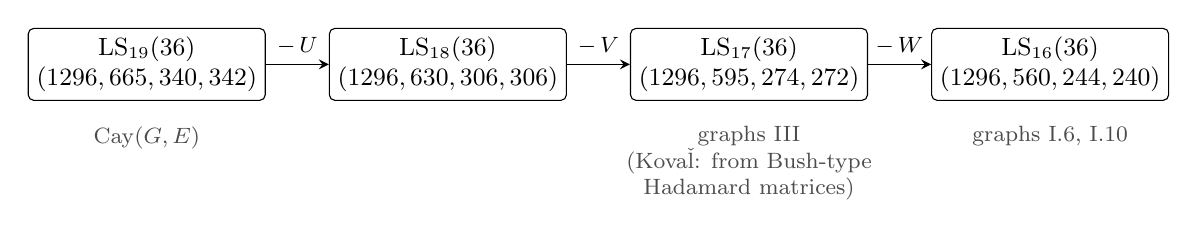
\begin{tikzpicture}[box/.style={draw,rounded corners=2pt,align=center,inner sep=3pt,font=\small},
  arr/.style={->,>=stealth,semithick},lab/.style={font=\footnotesize,above},note/.style={font=\footnotesize,align=center,text=black!70}]
\node[box] (a) {$\LS_{19}(36)$\\ $(1296,665,340,342)$};
\node[box,right=8mm of a] (b) {$\LS_{18}(36)$\\ $(1296,630,306,306)$};
\node[box,right=8mm of b] (c) {$\LS_{17}(36)$\\ $(1296,595,274,272)$};
\node[box,right=8mm of c] (d) {$\LS_{16}(36)$\\ $(1296,560,244,240)$};
\draw[arr] (a) -- node[lab] {$-\,U$} (b);
\draw[arr] (b) -- node[lab] {$-\,V$} (c);
\draw[arr] (c) -- node[lab] {$-\,W$} (d);
\node[note,below=2mm of a] {$\Cay(G,E)$};
\node[note,below=2mm of c] {graphs III\\ (Kova\v{l}: from Bush-type\\ Hadamard matrices)};
\node[note,below=2mm of d] {graphs I.6, I.10};
\end{tikzpicture}
\caption{Deleting pairwise orthogonal spreads (Proposition~\ref{prop:spreads}). Each arrow replaces the connection set $E$ by $E\setminus U$ for a subgroup $U$ of order $36$, and $U,V,W$ meet pairwise in $\{0\}$. The graphs III and I.6, I.10 come from different sets $E$.}\label{fig:spreads}
\end{figure}

So an $\LS_{19}(36)$ graph with three pairwise orthogonal spreads exists (Figure~\ref{fig:spreads}), the configuration sought in~\cite[Section~4.10]{KovalMultiOrbit}. We have not checked whether $\Cay(G,E)$ also arises from a Bush-type Hadamard matrix, as the graphs considered there do. Kova\v{l}'s $\LS_{17}(36)$ graphs and our graphs III are obtained by the same two-spread deletion, the former from Bush-type Hadamard matrices and the latter inside an abelian group.

\subsection{Relation to known constructions}\label{sec:known}
We checked the constructions of Latin square and negative Latin square type PDSs that could apply to abelian groups of order $1296=2^4\cdot3^4$. None of them gives any of our three parameter sets.
\begin{itemize}
\item \emph{Partial congruence partitions.} In an abelian group of order $36^2$, a set of subgroups of order $36$ that intersect pairwise trivially has at most $\min(2^2+1,3^2+1)=5$ members~\cite{Ma1994}. So these give $\LS_r(36)$ only for $r\le5$.
\item \emph{Product constructions.} The product theorems for packings of Latin square and negative Latin square type PDSs~\cite[Theorems 3.15, 6.8, Corollaries 3.17, 6.10]{JedwabLi2021}, including Polhill's product construction~\cite{Polhill2008}, combine packings in groups $G_1$, $G_2$ of orders $n_1^2$, $n_2^2$ with $n_1n_2=n$. They give $\LS_r(n)$ or $\NL_r(n)$ only when $r$ is a multiple of $n/t$ with $t>1$ dividing $\gcd(n_1,n_2)$. For $n=36$ we have $\gcd(n_1,n_2)\le 6$, so $r$ is a multiple of $6$. Our values $r=16$ ($\LS$ and $\NL$) and $r=17$ ($\LS$) are not, and neither are the complementary values $21$, $19$ and $20$.
\item \emph{Momihara's families}~\cite[Theorems 1.4, 1.5]{Momihara2021} live in products of elementary abelian groups of orders $q_i^4$ with $2m\mid q_i+1$ for all $i$. For $1296=2^4\cdot3^4$ this would require $2m\mid 3$ and $2m\mid 4$, which is impossible.
\item \emph{Cyclotomy over products of finite fields.} The standard cyclotomy of Fern\'andez-Alcober, Kwashira and Mart\'\i nez~\cite{FKM2010} on $\F_{16}\times\F_{81}$ has order $e\mid\gcd(15,80)=5$. Its PDSs are unions of orbits of a subgroup $H\le\F_{16}^*\times\F_{81}^*$ of index $e$. For $e=1$ the orbits have sizes $1,15,80,1200$, so no union has size $560$, $592$ or $595$. For $e=5$ there are four choices of $H$, and an exhaustive check shows that none of the $40$ unions of $H$-orbits of size $560$ or $592$ is a PDS. No union of $H$-orbits has size $595$. More directly, the multiplicative stabilisers of our connection sets have order at most $20$ (Table~\ref{tab:classes}), whereas a union of $H$-orbits is invariant under $H$, which has order $1200/e\ge240$. Ott's generalisations~\cite{Ott2016b,Ott2016a} consider unions of cosets of $U=\{(x_1,x_2):\chi_1(x_1)\chi_2(x_2)=1\}$, together with $U$-orbits of non-units, for multiplicative characters $\chi_i$ of order $d\mid q_i-1$. As Ott notes~\cite[Section~1]{Ott2016b}, these are exactly the subgroups of~\cite{FKM2010}. So here $d\mid5$, and the same two arguments exclude them. The new family of~\cite[Theorem~3]{Ott2016a} lives in groups of prime-power order $q^{2a+1}$.
\end{itemize}

%=====================================================================
\section{Verification}\label{sec:verification}
Each claimed graph was checked in three independent ways, and all checks pass.
\begin{enumerate}
\item A standalone program (plain Python, no external packages, no code shared with the search) builds $\Cay(G,D)$ with its own arithmetic in $\F_{16}$ and $\F_{81}$. It checks $D=-D$, $0\notin D$, the degree, and the number of common neighbours of all $839{,}160$ vertex pairs. It is run on Constructions~\ref{con:I}--\ref{con:III} exactly as printed above, and on the connection sets of all eighteen graphs.
\item Kova\v{l}'s independent verifier \texttt{verify\_srg.py}, from the data accompanying~\cite{KovalNew}, was run on the graph6 files of all eighteen graphs.
\item The spectra were computed numerically, and isomorphism classes and automorphism groups were computed with nauty~\cite{McKayPiperno2014}.
\end{enumerate}

%=====================================================================
\subsection*{Use of AI systems}
The search programs, the verification programs, the figures and a first draft of this text were produced in collaboration with an AI assistant (Claude Opus 5.5, Anthropic). All results were checked as described in Section~\ref{sec:verification}.

\subsection*{Data availability}
The connection sets of all graphs, the graphs in graph6 format, the standalone builders and verifiers, an interactive visualisation, and the search code are available at \url{https://github.com/dylan-plummer/srg1296}.

{\small
\setlength{\bibsep}{0pt plus 1pt}
\bibliographystyle{plainnat}
\bibliography{refs}
}

\end{document}
